%20 min preso!
\documentclass[xcolor=table]{beamer}
\usepackage{beamerthemesplit}
\usepackage{wrapfig}
\usetheme{SPbGU}
\usepackage{pdfpages}
\usepackage{amsmath}
\usepackage{cmap}
\usepackage[T2A]{fontenc}
\usepackage[utf8]{inputenc}
\usepackage[english]{babel}
\usepackage{indentfirst}
\usepackage{amsmath}
\usepackage{tikz}
\usepackage{multirow}
\usepackage[noend]{algpseudocode}
\usepackage{algorithm}
\usepackage{algorithmicx}
\usepackage{fancyvrb}
\usetikzlibrary{calc}
\usetikzlibrary{shapes,arrows}
\usetikzlibrary{arrows,automata}
\usetikzlibrary{positioning}

\usepackage{tabularx}
\newcolumntype{Y}{>{\raggedleft\arraybackslash}X}

\renewcommand{\thealgorithm}{}

\newtheorem{mytheorem}{Theorem}
\renewcommand{\thealgorithm}{}

\newcommand{\tikzmark}[1]{\tikz[overlay,remember picture] \node (#1) {};}
\def\Put(#1,#2)#3{\leavevmode\makebox(0,0){\put(#1,#2){#3}}}

\newcommand{\ltz}{$< 1$}


\tikzset{
    state/.style={
           rectangle,
           rounded corners,
           draw=black, very thick,
           minimum height=2em,
           inner sep=2pt,
           text centered,
           },
}

\beamertemplatenavigationsymbolsempty

\title[JBR PLT lab]{Лаборатория языковых инструментов}
\subtitle[]{Группа формальных языков}
% То, что в квадратных скобках, отображается в левом нижнем углу.
\institute[JetBrains Research]{
JetBrains Research, Лаборатория языковых инстументов \\
Санкт-Петербургский Государственный Университет
}

% То, что в квадратных скобках, отображается в левом нижнем углу.
\author[Семён Григорьев]{Семён Григорьев}

\date{4 октября, 2019}

\begin{document}
{
\begin{frame}[fragile]
  \begin{table}
  \centering
  \begin{tabularx}{\linewidth}{YcX}
    
\includegraphics[height=1.5cm]{pictures/jetbrainsResearch.pdf} \hfill
    & \begin{minipage}[t]{0.3\textwidth}
      \end{minipage}
    & \hfill 
\includegraphics[height=1.5cm]{pictures/SPbGU_Logo.png}
  \end{tabularx}
  \end{table}
  \titlepage
\end{frame}
}

\begin{frame} \frametitle{Лаборатория языковых инструментов}
  \begin{itemize}
        \item \textbf{Петергоф, Мат-Мех, 3248}
        \item Совместный проект JetBrains и кафедры системного программтирования СПбГУ: \textbf{\url{https://research.jetbrains.org/groups/plt_lab}}
        \item Исследования в области языков программирования: модели памяти, теория формальных языков, верификация, парадигмы программирования (функциональное, реляционное) и т.д.
        \item Руководитель: Дмитрий Юрьевич Булычев
  \end{itemize}

\end{frame}

\begin{frame}[fragile] \frametitle{Как к нам попасть}
    \begin{enumerate}
      \item Прийти на семинар (каждый понедельник в 17.30, аудитория 3248)
      \item Пообщаться с людьми
      \item Найти интересную для себя тему и взять курсовую
    \end{enumerate}
\end{frame}

\begin{frame}[fragile] \frametitle{Немного фамилий}
Сотрудники, аспиранты, студенты нашей лаборатории
    \begin{enumerate}
      \item Антон Подкопаев
      \item Даниил Березун
      \item Екатерина Вербицкая
      \item Никита Мишин
      \item Полина Лунина
      \item Юлия Сусанина
      \item Косарев Дмирий
      \item Мордвинов Дмитрий
      \item \dots
    \end{enumerate}
\end{frame}


\begin{frame}[fragile] \frametitle{Графовые базы данных и формальные языки}
  \begin{minipage}[m]{0.45\linewidth}
  \raisebox{-0.5\totalheight}{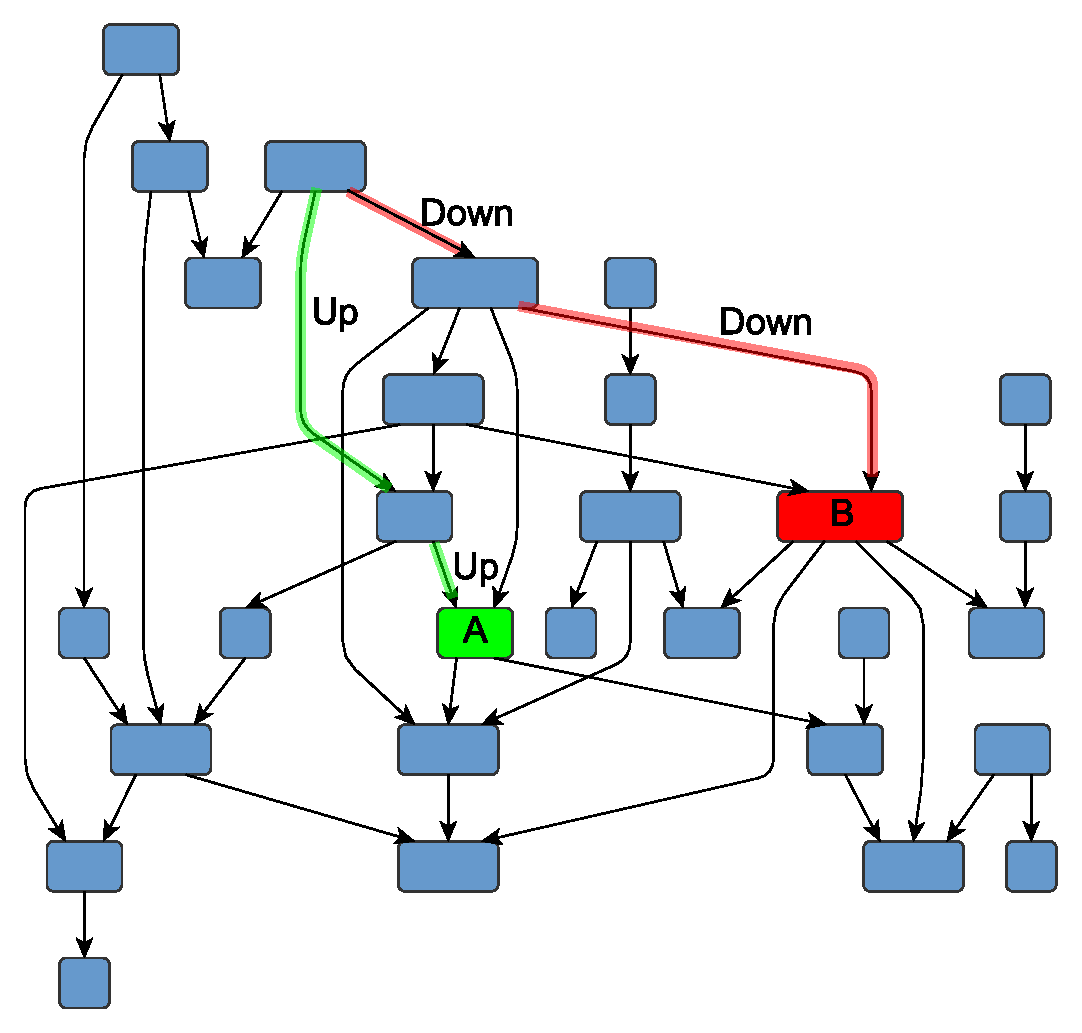
\includegraphics[width=\textwidth]{pictures/hierarchical.pdf}}
  \end{minipage}\hfill
  \begin{minipage}[m]{0.5\linewidth}
  Навигация по графу
  \begin{itemize}
        \item Правда ли, что узлы \textbf{A} и \textbf{B} находятся на одном уровне иерархии?
        \item Есть ли в графе пути вида $\textbf{Up}^n \, \textbf{Down}^n$?
        \item Найти все пути вида $\textbf{Up}^n \, \textbf{Down}^n$, начинающиеся в узле \textbf{A}
  \end{itemize}

  \end{minipage}
\end{frame}

\begin{frame} \frametitle{Поиск путей с ограничениями в терминах формальных языков}
\begin{itemize}
\item Конечный ориентированный граф с метками на рёбрах $\mathcal{G} = (V,E,L)$
\item Путь --- это слово в алфавите $L$ $\omega(p) = \omega(v_0 \xrightarrow{l_0} v_1 \xrightarrow{l_1} \dots \xrightarrow{l_{n-1}} v_n ) = l_0 \cdot l_1 \cdot \ldots \cdot l_{n-1}$
\item Язык $\mathcal{L}$ (над алфавитом $L$)
\end{itemize}
\pause
\begin{itemize}
  \item Задача достижимости: $Q=\{(v_i,v_j) \ | \ \exists p = v_i \dots v_j, \omega(p) \in \mathcal{L}\}$
  \item Задача поиска путей: $Q=\{p \ | \ \omega(p) \in \mathcal{L}\}$
  \begin{itemize}
    \item Один путь, все пути, кратчайший путь\dots
  \end{itemize}
\end{itemize}

\end{frame}

\begin{frame} \frametitle{Поиск путей с контекстно-свободными ограничениями}
\begin{itemize}
\item $\mathcal{L}$ --- контекстно-свободный язык (КС язык)
\item $G_{\mathcal{L}} = (N,\Sigma,R,S)$
\item Задача достижимости: $Q=\{(v_i,v_j) \ | \ \exists p = v_i \dots v_j, S \xrightarrow[G_{\mathcal{L}}]{*} \omega(p) \}$
\item Задача поиска путей: $Q=\{p \ | \ S \xrightarrow[G_{\mathcal{L}}]{*} \omega(p)\}$
\end{itemize}

\end{frame}

\begin{frame} \frametitle{Пример КС запроса}
\begin{center}
  \begin{tabular}{  c  c  }
      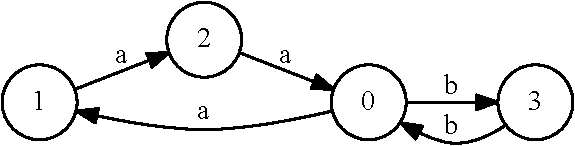
\includegraphics[width=0.45\textwidth]{pictures/input.pdf}
      &
  $

  \begin{array}{rl}
     & S \rightarrow a \ S \ b \\
     & S \rightarrow Middle \\
     & Middle \rightarrow a \ b
  \end{array}

  $
  \\
  Входной граф
  &
  Запрос: язык $\{a^nb^n \ | \ n > 0 \}$ 

  \end{tabular}

\end{center}

\pause

\vspace{0.5cm}
Пример путей: \\
$2 \xrightarrow{a} 0 \xrightarrow{b} 3$ \\
$1 \xrightarrow{a} 2 \xrightarrow{a} 0 \xrightarrow{b} 3 \xrightarrow{b} 0$ \\
$p_1 = 0 \xrightarrow{a} 1 \xrightarrow{a} 2 \xrightarrow{a} 0 \xrightarrow{b} 3 \xrightarrow{b} 0 \xrightarrow{b} 3$ \\
$p_2 = 0 \xrightarrow{a} 1 \xrightarrow{a} 2 \xrightarrow{a} 0 \xrightarrow{a} 1 \xrightarrow{a} 2 \xrightarrow{a} 0 \xrightarrow{b} 3 \xrightarrow{b} 0 \xrightarrow{b} 3 \xrightarrow{b} 0 \xrightarrow{b} 3 \xrightarrow{b} 0$ \\
$\dots$

\end{frame}

\begin{frame}[fragile] \frametitle{Задачи}
  \begin{enumerate}
    \item Реализовать Quad-tree представление разреженных матриц и операции над ним (сложение, умножение) на GPGPU (CUDA C / OpenCL C / С++)
    \pause
    \item Создать набор данных для экспериментального исследования алгоритмов
    \pause
    \item Умножение битовых матриц и матриц в F2, и интеграция с M4RI: \small{\url{https://github.com/SokolovYaroslav/CFPQ-on-GPGPU/issues/33}}
    \pause
    \item Разработать алгоритм динамического обновления результатов запроса
    \pause
    \item Реализовать различные алгоритмы на GraphBLAST: \url{https://github.com/gunrock/graphblast/issues/2}
  \end{enumerate}
\end{frame}

\begin{frame}
\frametitle{Контакты}
\begin{itemize}
  \item Semyon Grigorev:
    \begin{itemize}
      \item \href{mailto:rsdpisuy@gmail.com}{rsdpisuy@gmail.com}
      \item \href{mailto:Semyon.Grigorev@jetbrains.com}{Semyon.Grigorev@jetbrains.com}
    \end{itemize}
\end{itemize}
\end{frame}


\end{document}
